As stated before, we plan to split the work related with this PhD project in two parts: 
\begin{enumerate*}
\item the first part, focused on the framework allocated within each robot; and
\item the second part, focused on the choreography of a team of robots.
\end{enumerate*}

Therefore, our future work will be focused on trying to find an answer to the RQ2.
In order to achieve it, a detailed study of the current state of the art of features involved with multi-robot choreography such as emergent properties or collaborative strategies must be performed.
Nevertheless, since our plan is to continously integrate all the obtained knowledge into the research the framework developed during the first division of the project will be used and tested through this part as well.
Furthermore, due to the tools created for the robot orchestration will be tested on real robots we still will need to deploy the software platform and its functionalities on each of them.
An architectural overview of the whole research is depicted in Figure~\ref{fig:overview}.
\sergio{fix figure adding dotted lines! rename to collective adaptation!}
In this figure the expected final system is represented in a schematic way.
It represents blocks that emulates the contents of each robot that are unfolded, representing a team of robots.
The communication methodology is also represented in the figure, explaining how the robots will communicate.
Then, the properties that we plan to study in order to perform the orchestration are also depicted on top of the previous explained blocks. 
In the following we explain those properties.

\begin{figure}[!t]
\begin{center}
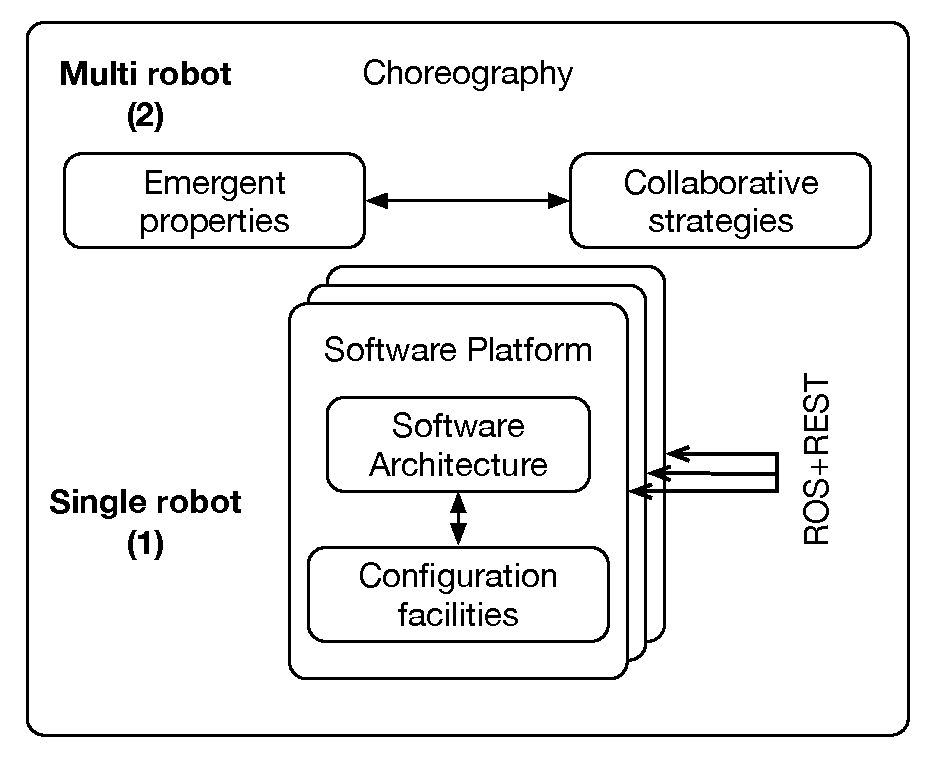
\includegraphics[width=1\linewidth]{Figures/researchv2.pdf}
\caption{Architectural overview of the final system.}
\label{fig:overview}
\end{center}
\end{figure}